\chapter{РАЗРАБОТКА МЕТОДИКИ ПО СОЗДАНИЮ ВЫСОКОНАГРУЖЕННЫХ ВЕБ-ПРИЛОЖЕНИЯХ} \label{ch3}

 
	
\section{Определение требований} \label{ch3:sec1}

В данной работе одной задачей является исследование основных источников угроз высоконагруженных веб-приложения. Основные угрозы для веб-приложений были рассмотрены и выявлены в первой главе настоящей работы. Так же обозначены специфичные угрозы для них.

Направлений разработки высоконагруженных веб-приложений – множество, каждое из них обладает своими потенциальными угрозами. Связанно это с тем, что высокие нагрузки – понятие относительное, как говорилось в первой главе. Однако все системы с высокой нагрузкой объединяет требовательность в ресурсах, как вычислительных, так и хранилищ. На основе этого сформируем методику разработки высоконагруженных систем, которая обобщит разные направления разработки, однако акцентирует внимание на обеспечении наименьшего показателя реакции системы.



\section{Разработка рекомендаций} \label{ch3:sec2}

Основные угрозы, нарушающие корректную работоспособность веб-приложения, были описаны в первой главе текущей работы. Так же были определены основные виды данных приложений. Основываться на это и на результаты работы \cite{AmazonAn66:online}, а так же на проведённый анализ в рамках исследования, в целях минимизации уязвимостей рекомендуется:

\begin{itemize}[•]
	\item Продумать архитектуру, согласно которой будет реализовываться высоконагруженное веб-приложение;
	\item Создание маршрутной карты;
	\item Определится с механизмами аутентификации и авторизации;
	\item Проводить фильтрацию всей вводимой информации;
	\item Хранить данные в зашифрованном виде;
	\item Определить и использовать специализированные http заголовки;
	\item Ограничить SQL запросы;
	\item Реализовать взаимоисключающий доступ к ресурсам или директориям;
	\item Производить http опрос, для подтверждения наличия соединения.
\end{itemize}

%\FloatBarrier % заставить рисунки и другие подвижные (float) элементы остановиться

\section{Обоснование выбора инструментария} \label{ch3:sec3}

Для разработки прототипа приложения был определён следующий стек технологий.

Разработка серверной части:

\textbf{Node js}. В качестве серверного языка была выбрана платформа Node js. Основной причиной данного выбора является требованием со стороны заказчика. Однако для внесения ясности скажу, что node js основан на движке V8 от компании Google. Особенностью этого движка заключается в том, что он экономно расходует память, неплохо оптимизирован, дает функционал по профилированию процессора и памяти. Так же комьюнити по всему миру трудятся над ним, что в свою очередь стремительно улучает его.

\textbf{Express.js} – фреймворк, созданный для упрощения разработки для веб-приложений и API. Был выбран в качестве дополнения при разработке сервера. Express уже является стандартным каркасом для разработчиков веб-приложений, так как упрощает базовые функции предоставляемые из коробки Node js.

\textbf{PostgreSQL} была выбрана в качестве СУБД. Связанно это с тем, что она предоставляется по бесплатной лицензии в плоть до коммерческого использования, поддерживает сложные запросы (выходящие за рамки базовых SQL запросов), позволяет пользователям самим определять и писать свои функции и типы данных и это является одним из требования договора.

\textbf{Socket.io}. На основе исследования, проведенного во второй главе настоящей работы, для обеспечения взаимодействия между клиентами и сервером в режиме реального времени была выбрана библиотека socket.io. Она поддерживает передачу пользовательских событий, производит проверку на подключен ли пользователь, а так же производит автоматическое переподключение.

Для разработки клиентской части выбрали:

\textbf{React} – это библиотека с открытым исходным кодом для разработки пользовательского интерфейса. React в основном используется для разработки одностраничных и мобильных приложений. Связанно это с тем, что react реализует эффективную логику обновления узлов DOM. Происходит это из-за виртуального DOM (VDOM), где виртуальное представление пользовательского интерфейса хранится в памяти и синхронизируется с настоящим DOM при помощи процесса соглосования.

\textbf{Easy-peasy}. Библиотека, предоставляет вам интуитивно понятный API для быстрого и удобного управления состоянием вашего приложения. Обеспечивает хранение и управление состояний приложения в глобальном объекте (store).

\textbf{Material-ui} – это библиотека, которая позволяет создавать приложения в стиле Google Material Design с использованием компонентов React. Она упрощает веб-разработку, создание привлекательных пользовательских интерфейсов и одностраничных приложений.

\section{Практическая реализация} \label{ch3:sec4}

Реализуем прототип приложения, который будет демонстрировать аспекты методики, чтобы произвести апробацию методики. 

В качестве прототипа приложения для апробации методики было выбрано реализация специализированного приложения для формирования отчётов по данным с заездов парусных яхт в период тренировок. Цель приложения – получение табличных и графических отчётов.

Приложение должно обеспечивать возможность формировать отчёты на веб странице, а так же в формате pdf (Start report, XY report, Phases report, Performance report) по входящим данным. Кроме этого, хранить storage все рассчитанные данные для формирования отчётов на веб-странице.

Архитектура приложения Рис. \ref{fig:АpplicationАrchitecture} представляет собой взаимодействие серверной части на базе Node js, Express.js, базой данных PostgreSQL и стороннего модуля пред расчета данных и клиентской части, представленной React, библиотекой Material-ui, leaflet и хранилища на основе easy-peasy. 

\begin{figure}
	\centering
	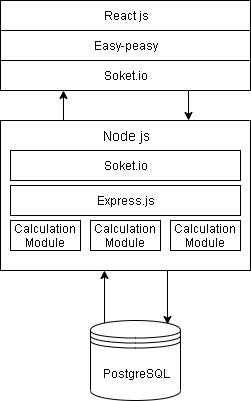
\includegraphics[scale=0.7]{my_folder/images/application architecture}
	\caption{Архитектура приложения}
	\label{fig:АpplicationАrchitecture}
\end{figure}

При подробном рассмотрении Рис. \ref{fig:АpplicationАrchitecture}, как ранее было сказано, библиотека React представляет клиентскую часть. Она обеспечивает масштабируемую разработку пользовательского интерфейса. Централизованное хранение информации реализовано с помощью библиотеки Easy-peasy. Она представляет информацию в виде глобального объект-хранилища. Взаимодействие с серверной частью происходит в рамках классического RESTful API. Реализовано с помощью отправки со стороны клиента Ajax-запросов, которые реализованы в Socket.io. Так же сам трансфер данных реализован с помощью Socket.io в рамках шаблона проектирования «издатель-подписчик». Это позволяет клиенту передавать данные заезда парусной яхты для расчёта отчётов на серверной стороне, которые он сохраняет в базе данных и отправляет обработанные данные клиенту для формирования отчётов на клиентской стороне. Для взаимодействия с PostgreSQL используется модуль pg\cite{pgnpm78:online} (неблокирующий клиент PostgreSQL для Node.js, не требующий дополнительных библиотек), позволяющий производить манипуляцию данных между базой данных и сервером. При получении данных на сервер определенного типа о необходимости расчёта данных, первоначально осуществляется поиск уже обработанных данных в СУБД PostgreSQL. Если же данные не найдены, то осуществляется расчёт отправленных пользователем данных. 

На Рис. \ref{fig:rgt_startReport} представлен пользовательский интерфейс приложения, разработанный с помощью Material-UI, а так же отчёт по Start report, показывающий инфографику начала стартового пути яхты.






\begin{figure}[hb]
	\centering
	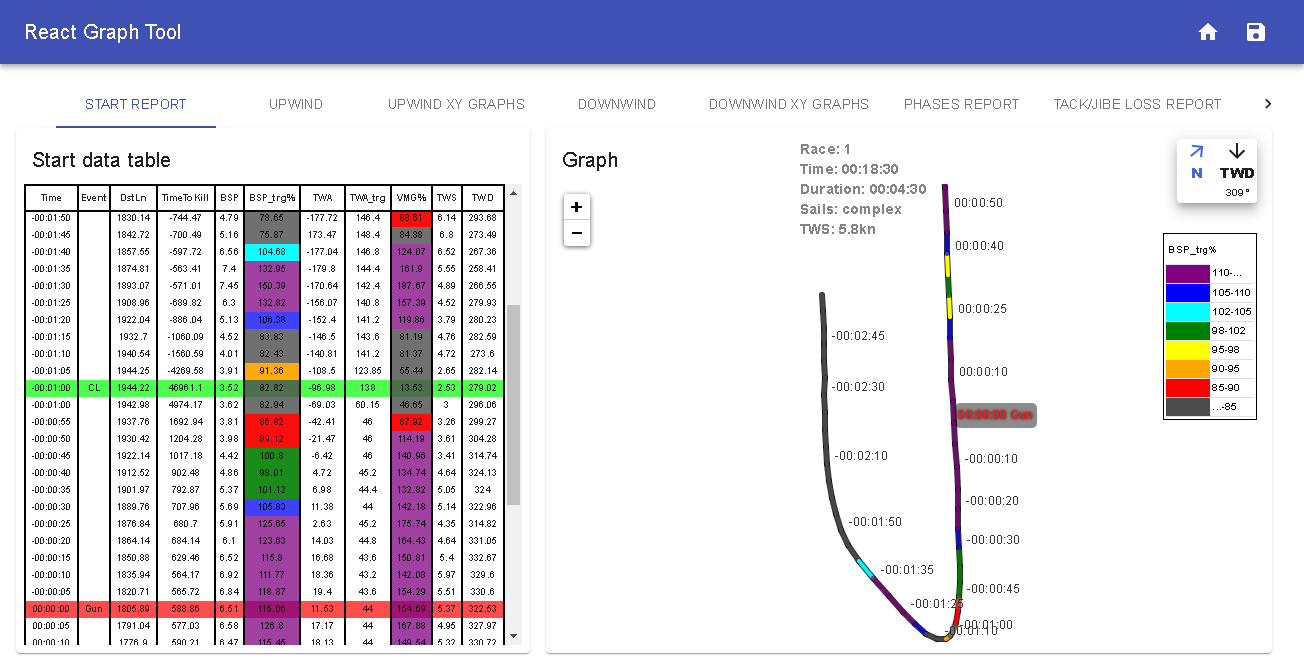
\includegraphics[scale=0.35]{my_folder/images/rgt_startReport}
	\caption{Пользовательский интерфейс вкладки Start report}
	\label{fig:rgt_startReport}
\end{figure}


На Рис. \ref{fig:rgt_XY} представлен, разработанный Upwind xy report, инфографику показывающие отношение характеристик к угловому ветру с помощью Material-UI.

\begin{figure}
	\centering
	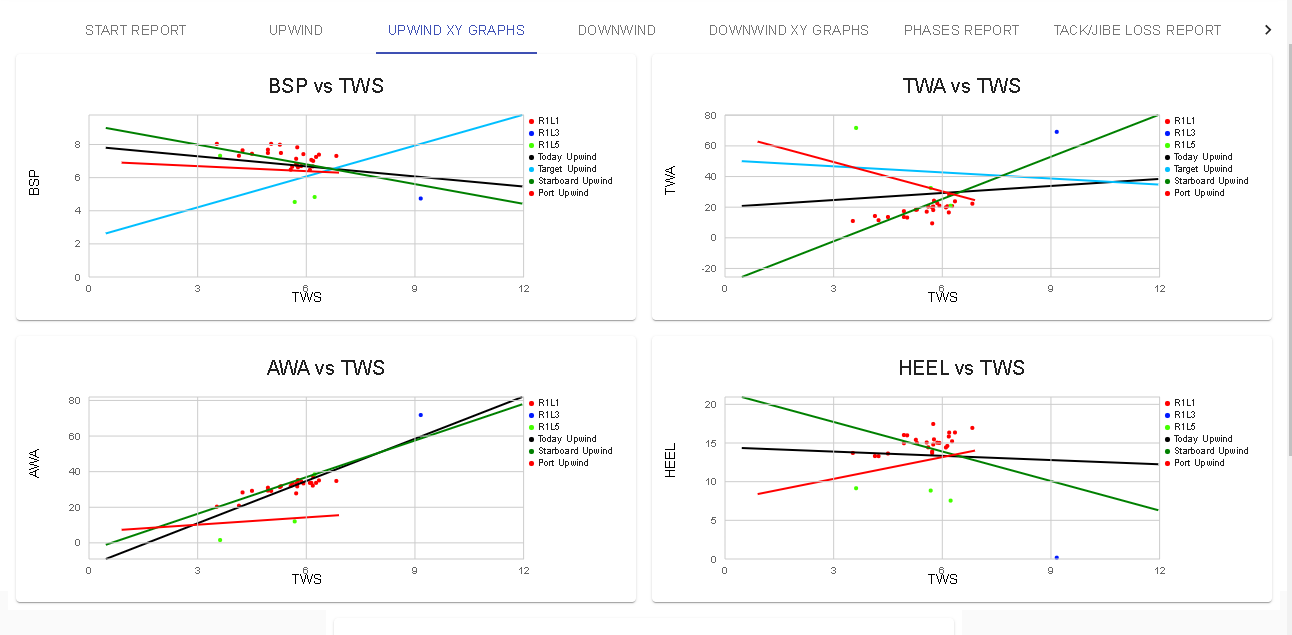
\includegraphics[scale=0.35]{my_folder/images/rgt_XY}
	\caption{Upwind XY report}
	\label{fig:rgt_XY}
\end{figure}

На Hис.\ref{fig:easypeasy} представлен срез глобального хранилища Easy-peasy.

\begin{figure}
	\centering
	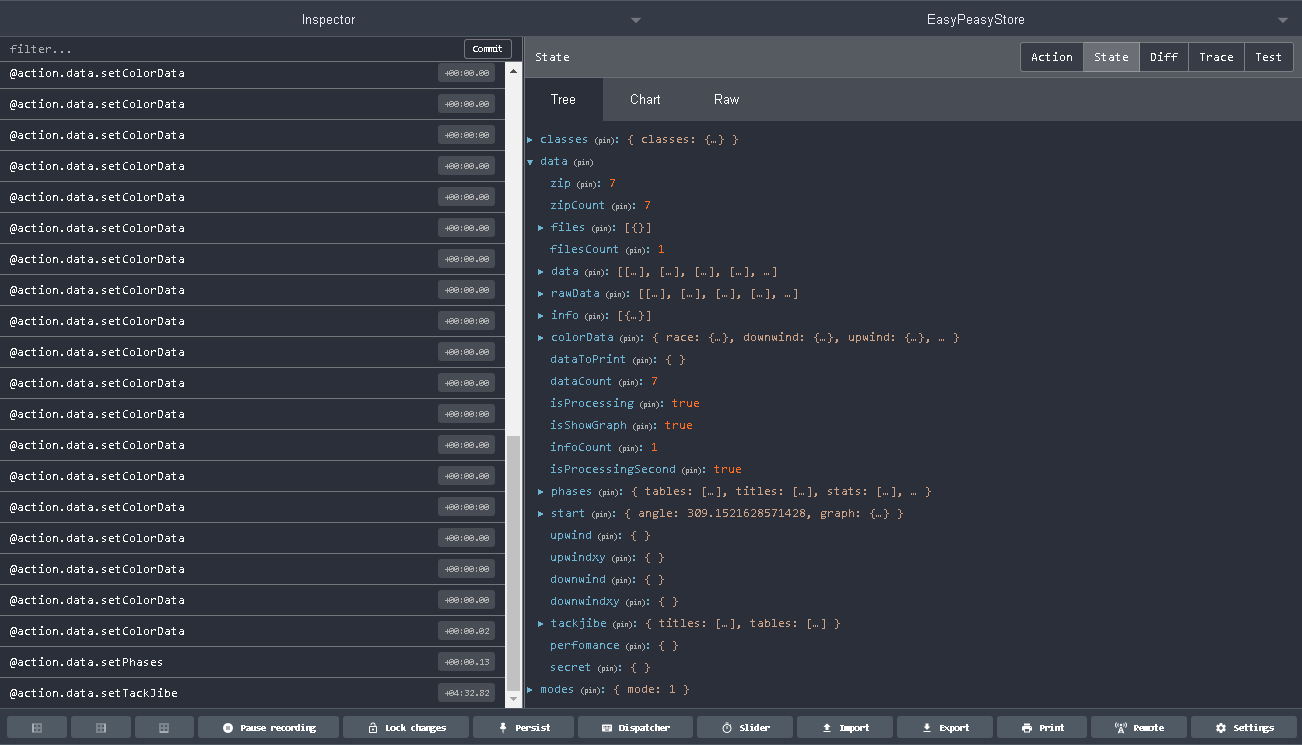
\includegraphics[scale=0.35]{my_folder/images/easypeasy}
	\caption{Upwind XY report}
	\label{fig:easypeasy}
\end{figure}

Приложения \cite{appendix:RGTMapGraph,appendix:RGTTableGraph,appendix:ReliseRESTfulAPI} демонстрируют код моделей табличного представления данных, графа пути. 

\newpage

\section{Сравнение с существующими технологиями} \label{ch3:sec5}

Тестирование прототипа реализовано с помощью фреймворка для нагрузочного тестирования Artillery.io. Он позволяет писать сценарии взаимодействия с приложением, а так же имитировать сложное поведение пользователя посредством нескольких шагов и транзакций с помощью циклов, условий на коде Javascript. Artillery.io удобно использовать для отладки сложных приложений, таких как транзакционные API, бэкэнд IoT,, бэкэнды онлайн игр и все виды сервисов с отслеживанием состояния.

Artillery.io обладает широким функционалом, который позволяет оценить время отклика, время задержки, количество запросов в секунду или отслеживать кастомные показатели с помощью кода Javascript.

Пример одного из использованных пользовательских сценариев показан:

\begin{lstlisting}
{
config:
	  target: "https://localhost:3000"
	  phases:
	- duration: 1000
		  arrivalRate: 1 
	  payload:
		  path: "Report_2020_05_13_11_59_01.fsr"
		  fields:
			- "files"
scenarios:
	- name: "Show start graph"
	  flow:
		- post:
			  url: "/api/start-report"
			  body: "file={{ keywords }}"
		- get:
			  url: "/start-report"
		- think: 500
\end{lstlisting}

Каждую секунду в течение 1000 секунд новый виртуальный пользователь отправляет файл из поля fields.file, пост запросом, на отображение стартовой страницы и остаётся в открытом соединении в течение 500 секунд.

Artillery.io предоставляет множество метрик для оценки тестов. Одни из них - количество выполненных запросов. Они являются количеством отправленных HTTP-запросов и ответов или сообщений от WebSocket. Так же число отправленных запросов в секунду. Является средним количеством запросов в секунду, выполненных за предыдущие 10 секунд (или в течение всего теста). Задержка запроса в миллисекундах. Значения p95 и p99, которые показывают максимальный предел задержки у 99 и 95 соответственно процентов запросов (к примеру, для 95 - показывает, что из 100 запросов 95-и запросам потребовалось меньше или равное 450мс).

Для сравнения с аналогами было принято решение использовать фреймворк artillery.io для проведения нагрузочного тестирования приложений B\&G sailing features и Sailwave на основе API Pusher.

\begin{table}
	\caption{Результаты нагрузочного тестирования}
	\label{loadTestResult}
	\begin{tabularx}{\linewidth}{|X|X|X|X|X|X|}
		\hline
		& Request latency (min) & Request latency (max) & Request latency (median) & P95 & P99\\
		\hline
		B\&G sailing features & 121 мс & 135 мс & 127 мс & 123 мс & 133 мс \\
		\hline
		Sailwave & (только Desktop) & (только Desktop) & (только Desktop) & (только Desktop) & (только Desktop)\\
		\hline
		Прототип приложения & 128 мс & 169 мс & 143 мс & 132 мс & 144 мс\\
		\hline
	\end{tabularx}
\end{table}

\begin{table}
	\caption{Таблица сравнения программ}
	\label{TableOfCmpPrograms}
	\begin{tabularx}{\linewidth}{|X|X|X|X|}
		\hline
		& Вид распространения & Цена & Функционал\\
		\hline
		B\&G sailing features & Desktop/ lite web & От 700\$ и может больше 2000\$ в зависимости от решения & Start report,
		Phase report,
		XY report,
		Tack/Jibe Loss report\\
		\hline
		Sailwave & Desktop & Free &Phase report,
		XY report,
		Tack/Jibe Loss report\\
		\hline
		Прототип приложения & web & Free & Start report,
		Phase report,
		XY report,
		Tack/Jibe Loss report,
		Perfomances\\
		\hline
	\end{tabularx}
\end{table}

\newpage

\section{Выводы} \label{ch3:conclusion}

В данной главе была сформулирована методика, предполагающая выполнение последовательности действий для сокращения угроз. Так же был определен стек для разработки прототипа приложения. Прототип специализированного веб-приложения для формирования отчётов по данным с заездов парусных яхт в период тренировок был разработан. Так же данный прототип подвергся нагрузочному тестированию. Были созданы тесты, которые имитируют посещение веб-приложения виртуальными пользователями. Нагрузочное тестирование показало, что прототип уступает по показателям, однако результаты можно считать сопоставимыми с результатами коммерческие аналогов, из чего следует, что предложенный архитектурный подход можно считать приемлемым.


%% Вспомогательные команды - Additional commands
%
%\newpage % принудительное начало с новой страницы, использовать только в конце раздела
%\clearpage % осуществляется пакетом <<placeins>> в пределах секций
%\newpage\leavevmode\thispagestyle{empty}\newpage % 100 % начало новой страницы